\documentclass{article}\usepackage[]{graphicx}\usepackage[]{color}
%% maxwidth is the original width if it is less than linewidth
%% otherwise use linewidth (to make sure the graphics do not exceed the margin)
\makeatletter
\def\maxwidth{ %
  \ifdim\Gin@nat@width>\linewidth
    \linewidth
  \else
    \Gin@nat@width
  \fi
}
\makeatother

\definecolor{fgcolor}{rgb}{0.345, 0.345, 0.345}
\newcommand{\hlnum}[1]{\textcolor[rgb]{0.686,0.059,0.569}{#1}}%
\newcommand{\hlstr}[1]{\textcolor[rgb]{0.192,0.494,0.8}{#1}}%
\newcommand{\hlcom}[1]{\textcolor[rgb]{0.678,0.584,0.686}{\textit{#1}}}%
\newcommand{\hlopt}[1]{\textcolor[rgb]{0,0,0}{#1}}%
\newcommand{\hlstd}[1]{\textcolor[rgb]{0.345,0.345,0.345}{#1}}%
\newcommand{\hlkwa}[1]{\textcolor[rgb]{0.161,0.373,0.58}{\textbf{#1}}}%
\newcommand{\hlkwb}[1]{\textcolor[rgb]{0.69,0.353,0.396}{#1}}%
\newcommand{\hlkwc}[1]{\textcolor[rgb]{0.333,0.667,0.333}{#1}}%
\newcommand{\hlkwd}[1]{\textcolor[rgb]{0.737,0.353,0.396}{\textbf{#1}}}%
\let\hlipl\hlkwb

\usepackage{framed}
\makeatletter
\newenvironment{kframe}{%
 \def\at@end@of@kframe{}%
 \ifinner\ifhmode%
  \def\at@end@of@kframe{\end{minipage}}%
  \begin{minipage}{\columnwidth}%
 \fi\fi%
 \def\FrameCommand##1{\hskip\@totalleftmargin \hskip-\fboxsep
 \colorbox{shadecolor}{##1}\hskip-\fboxsep
     % There is no \\@totalrightmargin, so:
     \hskip-\linewidth \hskip-\@totalleftmargin \hskip\columnwidth}%
 \MakeFramed {\advance\hsize-\width
   \@totalleftmargin\z@ \linewidth\hsize
   \@setminipage}}%
 {\par\unskip\endMakeFramed%
 \at@end@of@kframe}
\makeatother

\definecolor{shadecolor}{rgb}{.97, .97, .97}
\definecolor{messagecolor}{rgb}{0, 0, 0}
\definecolor{warningcolor}{rgb}{1, 0, 1}
\definecolor{errorcolor}{rgb}{1, 0, 0}
\newenvironment{knitrout}{}{} % an empty environment to be redefined in TeX

\usepackage{alltt}
\IfFileExists{upquote.sty}{\usepackage{upquote}}{}
\begin{document}



\begin{knitrout}
\definecolor{shadecolor}{rgb}{0.969, 0.969, 0.969}\color{fgcolor}\begin{kframe}
\begin{alltt}
\hlcom{## Load libraries}
\hlkwd{library}\hlstd{(splines)}
\hlkwd{library}\hlstd{(MASS)}

\hlcom{##source functions}
\hlkwd{source}\hlstd{(}\hlstr{"../functions.R"}\hlstd{)}
\end{alltt}
\end{kframe}
\end{knitrout}

\begin{knitrout}
\definecolor{shadecolor}{rgb}{0.969, 0.969, 0.969}\color{fgcolor}\begin{kframe}
\begin{alltt}
\hlstd{alts} \hlkwb{<-} \hlkwd{c}\hlstd{(}\hlstr{"alt_z_large"}\hlstd{,}\hlstr{"alt_t_large"}\hlstd{)}

\hlkwa{for}\hlstd{(alt} \hlkwa{in} \hlstd{alts)}
\hlstd{\{}
  \hlkwd{print}\hlstd{(alt)}
  \hlkwd{print}\hlstd{(}\hlstr{"I"}\hlstd{)}

  \hlkwd{load}\hlstd{(}\hlkwd{paste}\hlstd{(alt,}\hlstr{"simResults_1.RData"}\hlstd{,}\hlkwc{sep}\hlstd{=}\hlstr{"/"}\hlstd{))}
  \hlkwd{load}\hlstd{(}\hlkwd{paste}\hlstd{(alt,}\hlstr{"simResults_pi0x_thresh_1.RData"}\hlstd{,}\hlkwc{sep}\hlstd{=}\hlstr{"/"}\hlstd{))}
  \hlkwd{load}\hlstd{(}\hlkwd{paste}\hlstd{(alt,}\hlstr{"simResults_pi0x_Scott_emp_1.RData"}\hlstd{,}\hlkwc{sep}\hlstd{=}\hlstr{"/"}\hlstd{))}
  \hlkwd{load}\hlstd{(}\hlkwd{paste}\hlstd{(alt,}\hlstr{"simResults_pi0x_Scott_1.RData"}\hlstd{,}\hlkwc{sep}\hlstd{=}\hlstr{"/"}\hlstd{))}

  \hlkwd{plotMeanPi0}\hlstd{(pi0, pi0MeansVars, pi0hatScottMean,} \hlkwc{tme}\hlstd{=tme)}
  \hlkwd{legend}\hlstd{(}\hlstr{"topright"}\hlstd{,} \hlkwc{inset}\hlstd{=}\hlkwd{c}\hlstd{(}\hlopt{-}\hlnum{0.71}\hlstd{,}\hlnum{0}\hlstd{),}
         \hlkwc{legend}\hlstd{=}\hlkwd{c}\hlstd{(}\hlstr{"Truth"}\hlstd{,} \hlkwd{expression}\hlstd{(}\hlkwd{paste}\hlstd{(}\hlstr{"SLR ("}\hlstd{, lambda,} \hlstr{"=0.8)"}\hlstd{)),}
                  \hlkwd{expression}\hlstd{(}\hlkwd{paste}\hlstd{(}\hlstr{"SLR ("}\hlstd{, lambda,} \hlstr{"=0.9)"}\hlstd{)),}
                  \hlstr{"SLR (smoothed)"}\hlstd{,} \hlstr{"SLR (Scott)"}\hlstd{),}
         \hlkwc{col}\hlstd{=}\hlkwd{c}\hlstd{(}\hlstr{"black"}\hlstd{,} \hlstr{"orange"}\hlstd{,} \hlstr{"orange"}\hlstd{,} \hlstr{"orange"}\hlstd{,} \hlstr{"blue"}\hlstd{),} \hlkwc{bty}\hlstd{=}\hlstr{"n"}\hlstd{,}
         \hlkwc{lwd}\hlstd{=}\hlkwd{c}\hlstd{(}\hlnum{8}\hlstd{,}\hlnum{2}\hlstd{,}\hlnum{2}\hlstd{,}\hlnum{3}\hlstd{,}\hlnum{3}\hlstd{),} \hlkwc{lty}\hlstd{=}\hlkwd{c}\hlstd{(}\hlnum{1}\hlstd{,}\hlnum{3}\hlstd{,}\hlnum{2}\hlstd{,}\hlnum{1}\hlstd{,}\hlnum{1}\hlstd{),}
         \hlkwc{cex}\hlstd{=}\hlnum{1.2}\hlstd{,} \hlkwc{x.intersp}\hlstd{=}\hlnum{0.2}\hlstd{,} \hlkwc{y.intersp}\hlstd{=}\hlnum{1.0}\hlstd{)}

  \hlcom{#################################################################################}

    \hlkwd{print}\hlstd{(}\hlstr{"II"}\hlstd{)}

  \hlkwd{load}\hlstd{(}\hlkwd{paste}\hlstd{(alt,}\hlstr{"simResults_2.RData"}\hlstd{,}\hlkwc{sep}\hlstd{=}\hlstr{"/"}\hlstd{))}
  \hlkwd{load}\hlstd{(}\hlkwd{paste}\hlstd{(alt,}\hlstr{"simResults_pi0x_thresh_2.RData"}\hlstd{,}\hlkwc{sep}\hlstd{=}\hlstr{"/"}\hlstd{))}
  \hlkwd{load}\hlstd{(}\hlkwd{paste}\hlstd{(alt,}\hlstr{"simResults_pi0x_Scott_emp_2.RData"}\hlstd{,}\hlkwc{sep}\hlstd{=}\hlstr{"/"}\hlstd{))}
  \hlkwd{load}\hlstd{(}\hlkwd{paste}\hlstd{(alt,}\hlstr{"simResults_pi0x_Scott_2.RData"}\hlstd{,}\hlkwc{sep}\hlstd{=}\hlstr{"/"}\hlstd{))}

  \hlkwd{plotMeanPi0}\hlstd{(pi0, pi0Lin.MeansVars, pi0hatLin.ScottMean,} \hlkwc{tme}\hlstd{=tme)}
  \hlkwd{legend}\hlstd{(}\hlstr{"topright"}\hlstd{,} \hlkwc{inset}\hlstd{=}\hlkwd{c}\hlstd{(}\hlopt{-}\hlnum{0.71}\hlstd{,}\hlnum{0}\hlstd{),}\hlcom{##x=-0.2, y=0.45,##"bottomright", ##x=-100, y=0.3, }
         \hlkwc{legend}\hlstd{=}\hlkwd{c}\hlstd{(}\hlstr{"Truth"}\hlstd{,}
                  \hlkwd{expression}\hlstd{(}\hlkwd{paste}\hlstd{(}\hlstr{"SLR ("}\hlstd{, lambda,} \hlstr{"=0.8)"}\hlstd{)),}
                  \hlkwd{expression}\hlstd{(}\hlkwd{paste}\hlstd{(}\hlstr{"SLR ("}\hlstd{, lambda,} \hlstr{"=0.9)"}\hlstd{)),}
                  \hlstr{"SLR (smoothed)"}\hlstd{,}
                  \hlstr{"SLR (Scott)"}\hlstd{),}
         \hlkwc{col}\hlstd{=}\hlkwd{c}\hlstd{(}\hlstr{"black"}\hlstd{,}
               \hlkwd{rep}\hlstd{(}\hlstr{"orange"}\hlstd{,}\hlnum{3}\hlstd{),}
               \hlstr{"blue"}\hlstd{),}
         \hlkwc{bty}\hlstd{=}\hlstr{"n"}\hlstd{,}
         \hlkwc{lwd}\hlstd{=}\hlkwd{c}\hlstd{(}\hlnum{8}\hlstd{,}\hlnum{2}\hlstd{,}\hlnum{2}\hlstd{,}\hlnum{3}\hlstd{,}\hlnum{3}\hlstd{),} \hlkwc{lty}\hlstd{=}\hlkwd{c}\hlstd{(}\hlnum{1}\hlstd{,}\hlnum{3}\hlstd{,}\hlnum{2}\hlstd{,}\hlnum{1}\hlstd{,}\hlnum{1}\hlstd{),}
         \hlkwc{cex}\hlstd{=}\hlnum{1.2}\hlstd{,} \hlkwc{x.intersp}\hlstd{=}\hlnum{0.2}\hlstd{,} \hlkwc{y.intersp}\hlstd{=}\hlnum{1.0}\hlstd{)}

  \hlkwd{plotMeanPi0}\hlstd{(pi0, pi0Spl.MeansVars, pi0hatSpl.ScottMean,} \hlkwc{tme}\hlstd{=tme)}
  \hlkwd{legend}\hlstd{(}\hlstr{"topright"}\hlstd{,} \hlkwc{inset}\hlstd{=}\hlkwd{c}\hlstd{(}\hlopt{-}\hlnum{0.71}\hlstd{,}\hlnum{0}\hlstd{),}\hlcom{##x=-0.2, y=0.45,##"bottomright", ##x=-100, y=0.3, }
         \hlkwc{legend}\hlstd{=}\hlkwd{c}\hlstd{(}\hlstr{"Truth"}\hlstd{,}
                  \hlkwd{expression}\hlstd{(}\hlkwd{paste}\hlstd{(}\hlstr{"B-splines, 3 df ("}\hlstd{, lambda,} \hlstr{"=0.8)"}\hlstd{)),}
                  \hlkwd{expression}\hlstd{(}\hlkwd{paste}\hlstd{(}\hlstr{"B-splines, 3 df ("}\hlstd{, lambda,} \hlstr{"=0.9)"}\hlstd{)),}
                  \hlstr{"B-splines, 3 df (smoothed)"}\hlstd{,}
                  \hlstr{"B-splines, 3 df (Scott)"}\hlstd{),}
         \hlkwc{col}\hlstd{=}\hlkwd{c}\hlstd{(}\hlstr{"black"}\hlstd{,}
               \hlkwd{rep}\hlstd{(}\hlstr{"orange"}\hlstd{,}\hlnum{3}\hlstd{),}
               \hlstr{"blue"}\hlstd{),}
         \hlkwc{bty}\hlstd{=}\hlstr{"n"}\hlstd{,}
         \hlkwc{lwd}\hlstd{=}\hlkwd{c}\hlstd{(}\hlnum{8}\hlstd{,}\hlnum{2}\hlstd{,}\hlnum{2}\hlstd{,}\hlnum{3}\hlstd{,}\hlnum{3}\hlstd{),} \hlkwc{lty}\hlstd{=}\hlkwd{c}\hlstd{(}\hlnum{1}\hlstd{,}\hlnum{3}\hlstd{,}\hlnum{2}\hlstd{,}\hlnum{1}\hlstd{,}\hlnum{1}\hlstd{),}
         \hlkwc{cex}\hlstd{=}\hlnum{1.2}\hlstd{,} \hlkwc{x.intersp}\hlstd{=}\hlnum{0.2}\hlstd{,} \hlkwc{y.intersp}\hlstd{=}\hlnum{1.0}\hlstd{)}

    \hlcom{#################################################################################}

    \hlkwd{print}\hlstd{(}\hlstr{"III"}\hlstd{)}

  \hlkwd{load}\hlstd{(}\hlkwd{paste}\hlstd{(alt,}\hlstr{"simResults_3.RData"}\hlstd{,}\hlkwc{sep}\hlstd{=}\hlstr{"/"}\hlstd{))}
  \hlkwd{load}\hlstd{(}\hlkwd{paste}\hlstd{(alt,}\hlstr{"simResults_pi0x_thresh_3.RData"}\hlstd{,}\hlkwc{sep}\hlstd{=}\hlstr{"/"}\hlstd{))}
  \hlkwd{load}\hlstd{(}\hlkwd{paste}\hlstd{(alt,}\hlstr{"simResults_pi0x_Scott_emp_3.RData"}\hlstd{,}\hlkwc{sep}\hlstd{=}\hlstr{"/"}\hlstd{))}
  \hlkwd{load}\hlstd{(}\hlkwd{paste}\hlstd{(alt,}\hlstr{"simResults_pi0x_Scott_3.RData"}\hlstd{,}\hlkwc{sep}\hlstd{=}\hlstr{"/"}\hlstd{))}

  \hlkwd{plotMeanPi0}\hlstd{(pi0, pi0Lin.MeansVars, pi0hatLin.ScottMean,} \hlkwc{tme}\hlstd{=tme)}
  \hlkwd{legend}\hlstd{(}\hlstr{"topright"}\hlstd{,} \hlkwc{inset}\hlstd{=}\hlkwd{c}\hlstd{(}\hlopt{-}\hlnum{0.71}\hlstd{,}\hlnum{0}\hlstd{),}\hlcom{##x=-0.2, y=0.45,##"bottomright", ##x=-100, y=0.3, }
         \hlkwc{legend}\hlstd{=}\hlkwd{c}\hlstd{(}\hlstr{"Truth"}\hlstd{,}
                  \hlkwd{expression}\hlstd{(}\hlkwd{paste}\hlstd{(}\hlstr{"SLR ("}\hlstd{, lambda,} \hlstr{"=0.8)"}\hlstd{)),}
                  \hlkwd{expression}\hlstd{(}\hlkwd{paste}\hlstd{(}\hlstr{"SLR ("}\hlstd{, lambda,} \hlstr{"=0.9)"}\hlstd{)),}
                  \hlstr{"SLR (smoothed)"}\hlstd{,}
                  \hlstr{"SLR (Scott)"}\hlstd{),}
         \hlkwc{col}\hlstd{=}\hlkwd{c}\hlstd{(}\hlstr{"black"}\hlstd{,}
               \hlkwd{rep}\hlstd{(}\hlstr{"orange"}\hlstd{,}\hlnum{3}\hlstd{),}
               \hlstr{"blue"}\hlstd{),}
         \hlkwc{bty}\hlstd{=}\hlstr{"n"}\hlstd{,}
         \hlkwc{lwd}\hlstd{=}\hlkwd{c}\hlstd{(}\hlnum{8}\hlstd{,}\hlnum{2}\hlstd{,}\hlnum{2}\hlstd{,}\hlnum{3}\hlstd{,}\hlnum{3}\hlstd{),} \hlkwc{lty}\hlstd{=}\hlkwd{c}\hlstd{(}\hlnum{1}\hlstd{,}\hlnum{3}\hlstd{,}\hlnum{2}\hlstd{,}\hlnum{1}\hlstd{,}\hlnum{1}\hlstd{),}
         \hlkwc{cex}\hlstd{=}\hlnum{1.2}\hlstd{,} \hlkwc{x.intersp}\hlstd{=}\hlnum{0.2}\hlstd{,} \hlkwc{y.intersp}\hlstd{=}\hlnum{1.0}\hlstd{)}

  \hlkwd{plotMeanPi0}\hlstd{(pi0, pi0Spl.MeansVars, pi0hatSpl.ScottMean,} \hlkwc{tme}\hlstd{=tme)}
  \hlkwd{legend}\hlstd{(}\hlstr{"topright"}\hlstd{,} \hlkwc{inset}\hlstd{=}\hlkwd{c}\hlstd{(}\hlopt{-}\hlnum{0.71}\hlstd{,}\hlnum{0}\hlstd{),}\hlcom{##x=-0.2, y=0.45,##"bottomright", ##x=-100, y=0.3, }
         \hlkwc{legend}\hlstd{=}\hlkwd{c}\hlstd{(}\hlstr{"Truth"}\hlstd{,}
                  \hlkwd{expression}\hlstd{(}\hlkwd{paste}\hlstd{(}\hlstr{"B-splines, 3 df ("}\hlstd{, lambda,} \hlstr{"=0.8)"}\hlstd{)),}
                  \hlkwd{expression}\hlstd{(}\hlkwd{paste}\hlstd{(}\hlstr{"B-splines, 3 df ("}\hlstd{, lambda,} \hlstr{"=0.9)"}\hlstd{)),}
                  \hlstr{"B-splines, 3 df (smoothed)"}\hlstd{,}
                  \hlstr{"B-splines, 3 df (Scott)"}\hlstd{),}
         \hlkwc{col}\hlstd{=}\hlkwd{c}\hlstd{(}\hlstr{"black"}\hlstd{,}
               \hlkwd{rep}\hlstd{(}\hlstr{"orange"}\hlstd{,}\hlnum{3}\hlstd{),}
               \hlstr{"blue"}\hlstd{),}
         \hlkwc{bty}\hlstd{=}\hlstr{"n"}\hlstd{,}
         \hlkwc{lwd}\hlstd{=}\hlkwd{c}\hlstd{(}\hlnum{8}\hlstd{,}\hlnum{2}\hlstd{,}\hlnum{2}\hlstd{,}\hlnum{3}\hlstd{,}\hlnum{3}\hlstd{),} \hlkwc{lty}\hlstd{=}\hlkwd{c}\hlstd{(}\hlnum{1}\hlstd{,}\hlnum{3}\hlstd{,}\hlnum{2}\hlstd{,}\hlnum{1}\hlstd{,}\hlnum{1}\hlstd{),}
         \hlkwc{cex}\hlstd{=}\hlnum{1.2}\hlstd{,} \hlkwc{x.intersp}\hlstd{=}\hlnum{0.2}\hlstd{,} \hlkwc{y.intersp}\hlstd{=}\hlnum{1.0}\hlstd{)}

     \hlcom{#################################################################################}

    \hlkwd{print}\hlstd{(}\hlstr{"IV"}\hlstd{)}

  \hlkwd{load}\hlstd{(}\hlkwd{paste}\hlstd{(alt,}\hlstr{"simResults_4.RData"}\hlstd{,}\hlkwc{sep}\hlstd{=}\hlstr{"/"}\hlstd{))}
  \hlkwd{load}\hlstd{(}\hlkwd{paste}\hlstd{(alt,}\hlstr{"simResults_pi0x_thresh_4.RData"}\hlstd{,}\hlkwc{sep}\hlstd{=}\hlstr{"/"}\hlstd{))}
  \hlkwd{load}\hlstd{(}\hlkwd{paste}\hlstd{(alt,}\hlstr{"simResults_pi0x_Scott_emp_4.RData"}\hlstd{,}\hlkwc{sep}\hlstd{=}\hlstr{"/"}\hlstd{))}
  \hlkwd{load}\hlstd{(}\hlkwd{paste}\hlstd{(alt,}\hlstr{"simResults_pi0x_Scott_4.RData"}\hlstd{,}\hlkwc{sep}\hlstd{=}\hlstr{"/"}\hlstd{))}

  \hlkwd{plotMeanPi0}\hlstd{(pi0, pi0Lin.MeansVars, pi0hatLin.ScottMean,} \hlkwc{tme}\hlstd{=tme)}
  \hlkwd{legend}\hlstd{(}\hlstr{"topright"}\hlstd{,} \hlkwc{inset}\hlstd{=}\hlkwd{c}\hlstd{(}\hlopt{-}\hlnum{0.71}\hlstd{,}\hlnum{0}\hlstd{),}\hlcom{##x=-0.2, y=0.45,##"bottomright", ##x=-100, y=0.3, }
         \hlkwc{legend}\hlstd{=}\hlkwd{c}\hlstd{(}\hlstr{"Truth"}\hlstd{,}
                  \hlkwd{expression}\hlstd{(}\hlkwd{paste}\hlstd{(}\hlstr{"SLR ("}\hlstd{, lambda,} \hlstr{"=0.8)"}\hlstd{)),}
                  \hlkwd{expression}\hlstd{(}\hlkwd{paste}\hlstd{(}\hlstr{"SLR ("}\hlstd{, lambda,} \hlstr{"=0.9)"}\hlstd{)),}
                  \hlstr{"SLR (smoothed)"}\hlstd{,}
                  \hlstr{"SLR (Scott)"}\hlstd{),}
         \hlkwc{col}\hlstd{=}\hlkwd{c}\hlstd{(}\hlstr{"black"}\hlstd{,}
               \hlkwd{rep}\hlstd{(}\hlstr{"orange"}\hlstd{,}\hlnum{3}\hlstd{),}
               \hlstr{"blue"}\hlstd{),}
         \hlkwc{bty}\hlstd{=}\hlstr{"n"}\hlstd{,}
         \hlkwc{lwd}\hlstd{=}\hlkwd{c}\hlstd{(}\hlnum{8}\hlstd{,}\hlnum{2}\hlstd{,}\hlnum{2}\hlstd{,}\hlnum{3}\hlstd{,}\hlnum{3}\hlstd{),} \hlkwc{lty}\hlstd{=}\hlkwd{c}\hlstd{(}\hlnum{1}\hlstd{,}\hlnum{3}\hlstd{,}\hlnum{2}\hlstd{,}\hlnum{1}\hlstd{,}\hlnum{1}\hlstd{),}
         \hlkwc{cex}\hlstd{=}\hlnum{1.2}\hlstd{,} \hlkwc{x.intersp}\hlstd{=}\hlnum{0.2}\hlstd{,} \hlkwc{y.intersp}\hlstd{=}\hlnum{1.0}\hlstd{)}

  \hlkwd{plotMeanPi0}\hlstd{(pi0, pi0Spl.MeansVars, pi0hatSpl.ScottMean,} \hlkwc{tme}\hlstd{=tme)}
  \hlkwd{legend}\hlstd{(}\hlstr{"topright"}\hlstd{,} \hlkwc{inset}\hlstd{=}\hlkwd{c}\hlstd{(}\hlopt{-}\hlnum{0.71}\hlstd{,}\hlnum{0}\hlstd{),}\hlcom{##x=-0.2, y=0.45,##"bottomright", ##x=-100, y=0.3, }
         \hlkwc{legend}\hlstd{=}\hlkwd{c}\hlstd{(}\hlstr{"Truth"}\hlstd{,}
                  \hlkwd{expression}\hlstd{(}\hlkwd{paste}\hlstd{(}\hlstr{"B-splines, 3 df ("}\hlstd{, lambda,} \hlstr{"=0.8)"}\hlstd{)),}
                  \hlkwd{expression}\hlstd{(}\hlkwd{paste}\hlstd{(}\hlstr{"B-splines, 3 df ("}\hlstd{, lambda,} \hlstr{"=0.9)"}\hlstd{)),}
                  \hlstr{"B-splines, 3 df (smoothed)"}\hlstd{,}
                  \hlstr{"B-splines, 3 df (Scott)"}\hlstd{),}
         \hlkwc{col}\hlstd{=}\hlkwd{c}\hlstd{(}\hlstr{"black"}\hlstd{,}
               \hlkwd{rep}\hlstd{(}\hlstr{"orange"}\hlstd{,}\hlnum{3}\hlstd{),}
               \hlstr{"blue"}\hlstd{),}
         \hlkwc{bty}\hlstd{=}\hlstr{"n"}\hlstd{,}
         \hlkwc{lwd}\hlstd{=}\hlkwd{c}\hlstd{(}\hlnum{8}\hlstd{,}\hlnum{2}\hlstd{,}\hlnum{2}\hlstd{,}\hlnum{3}\hlstd{,}\hlnum{3}\hlstd{),} \hlkwc{lty}\hlstd{=}\hlkwd{c}\hlstd{(}\hlnum{1}\hlstd{,}\hlnum{3}\hlstd{,}\hlnum{2}\hlstd{,}\hlnum{1}\hlstd{,}\hlnum{1}\hlstd{),}
         \hlkwc{cex}\hlstd{=}\hlnum{1.2}\hlstd{,} \hlkwc{x.intersp}\hlstd{=}\hlnum{0.2}\hlstd{,} \hlkwc{y.intersp}\hlstd{=}\hlnum{1.0}\hlstd{)}
\hlstd{\}}
\end{alltt}
\begin{verbatim}
## [1] "alt_z_large"
## [1] "I"
## [1] "II"
## [1] "III"
## [1] "IV"
## [1] "alt_t_large"
## [1] "I"
## [1] "II"
## [1] "III"
## [1] "IV"
\end{verbatim}
\end{kframe}

{\centering 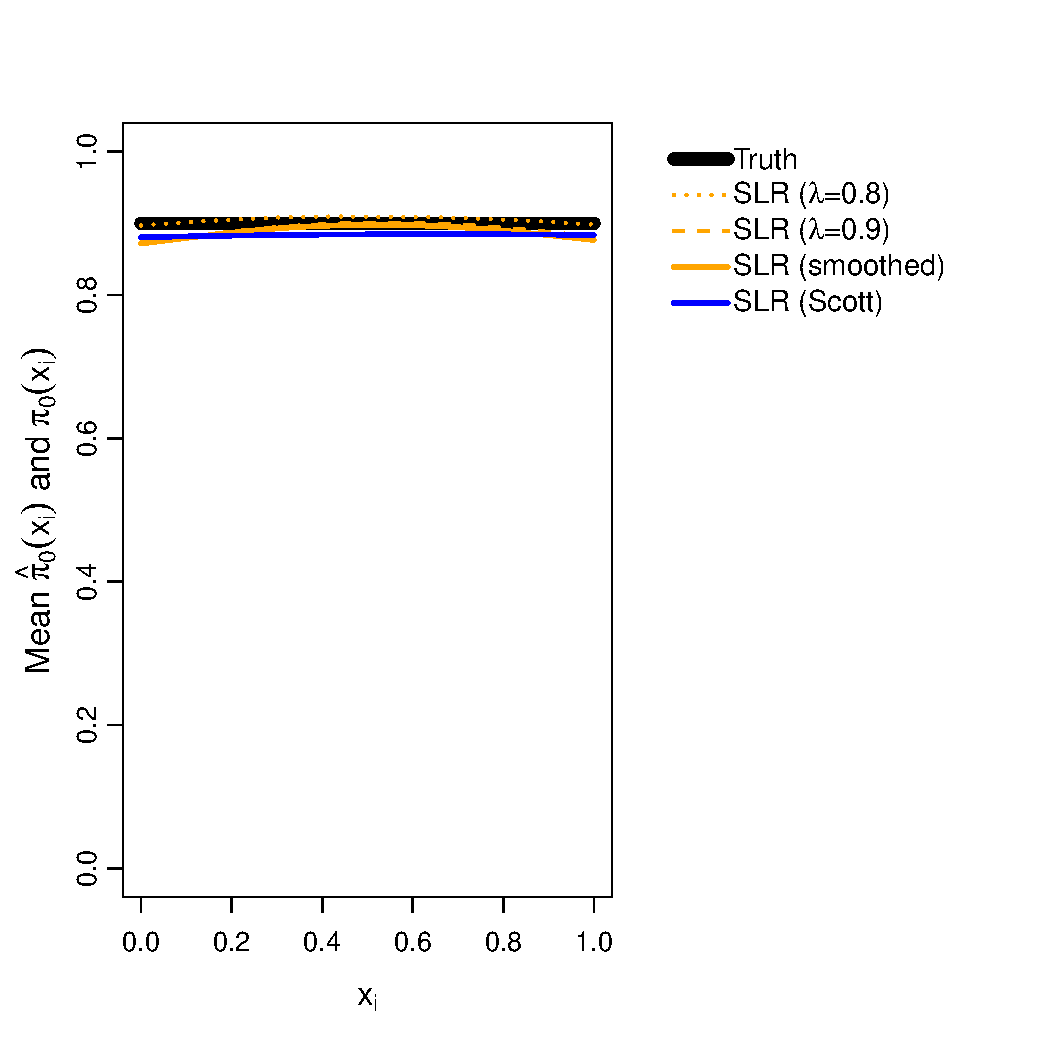
\includegraphics[width=\maxwidth]{Figures/unnamed-chunk-1-1} 
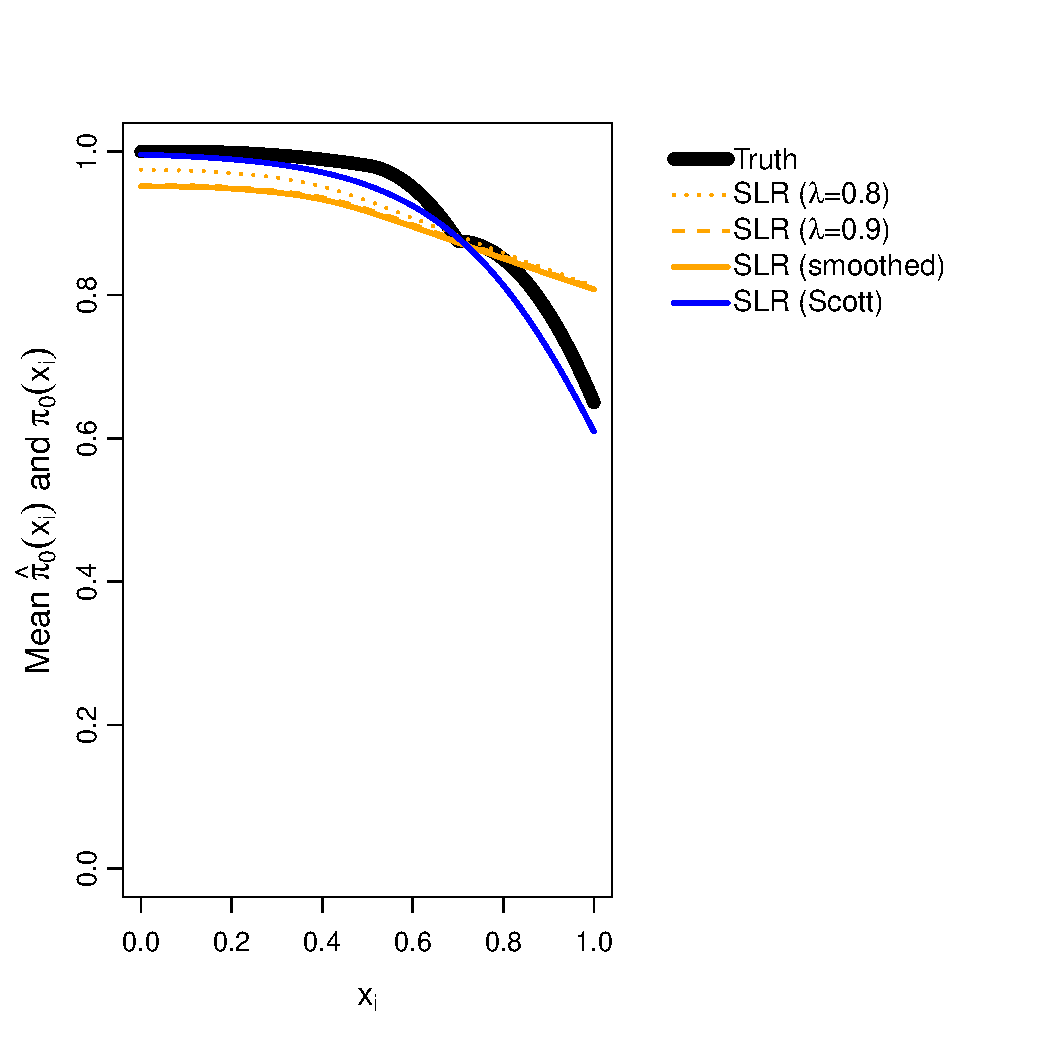
\includegraphics[width=\maxwidth]{Figures/unnamed-chunk-1-2} 
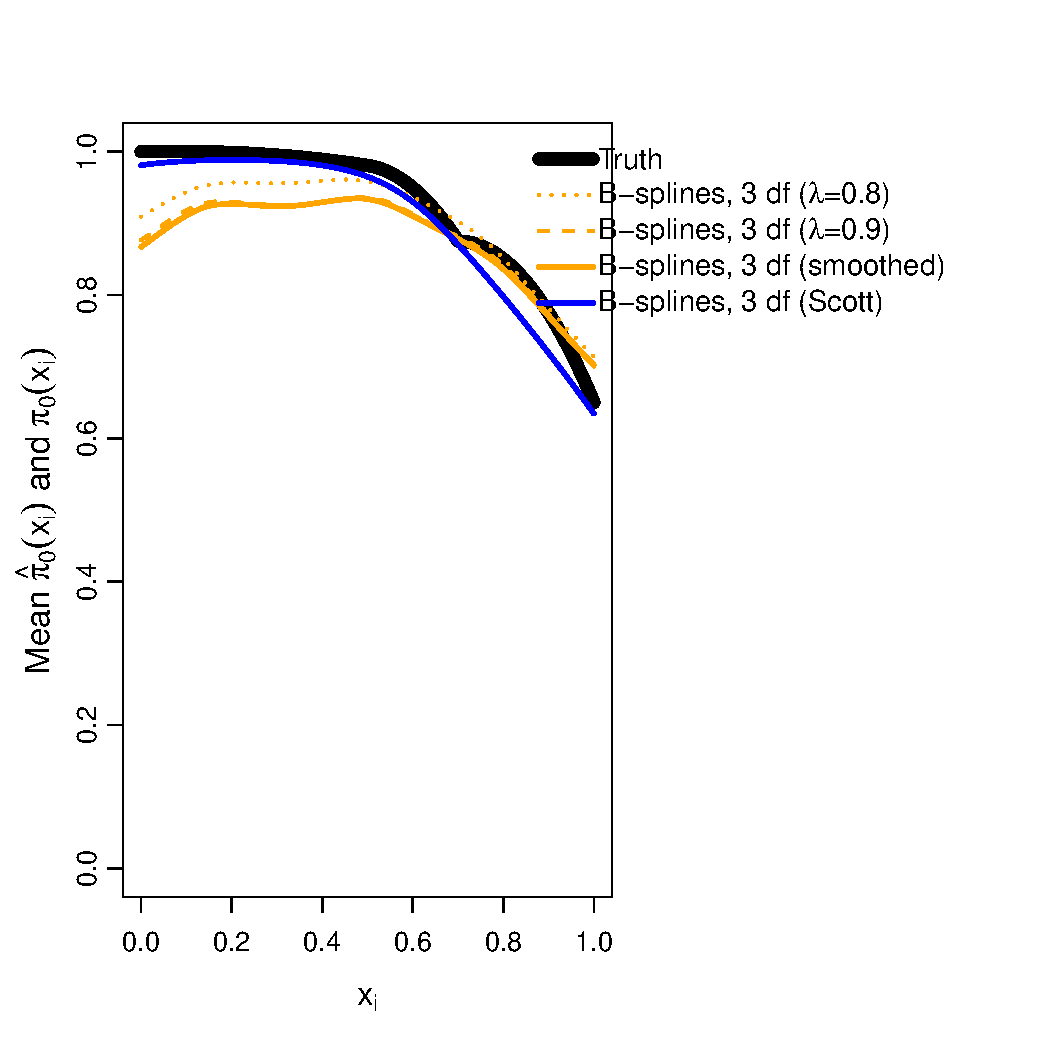
\includegraphics[width=\maxwidth]{Figures/unnamed-chunk-1-3} 
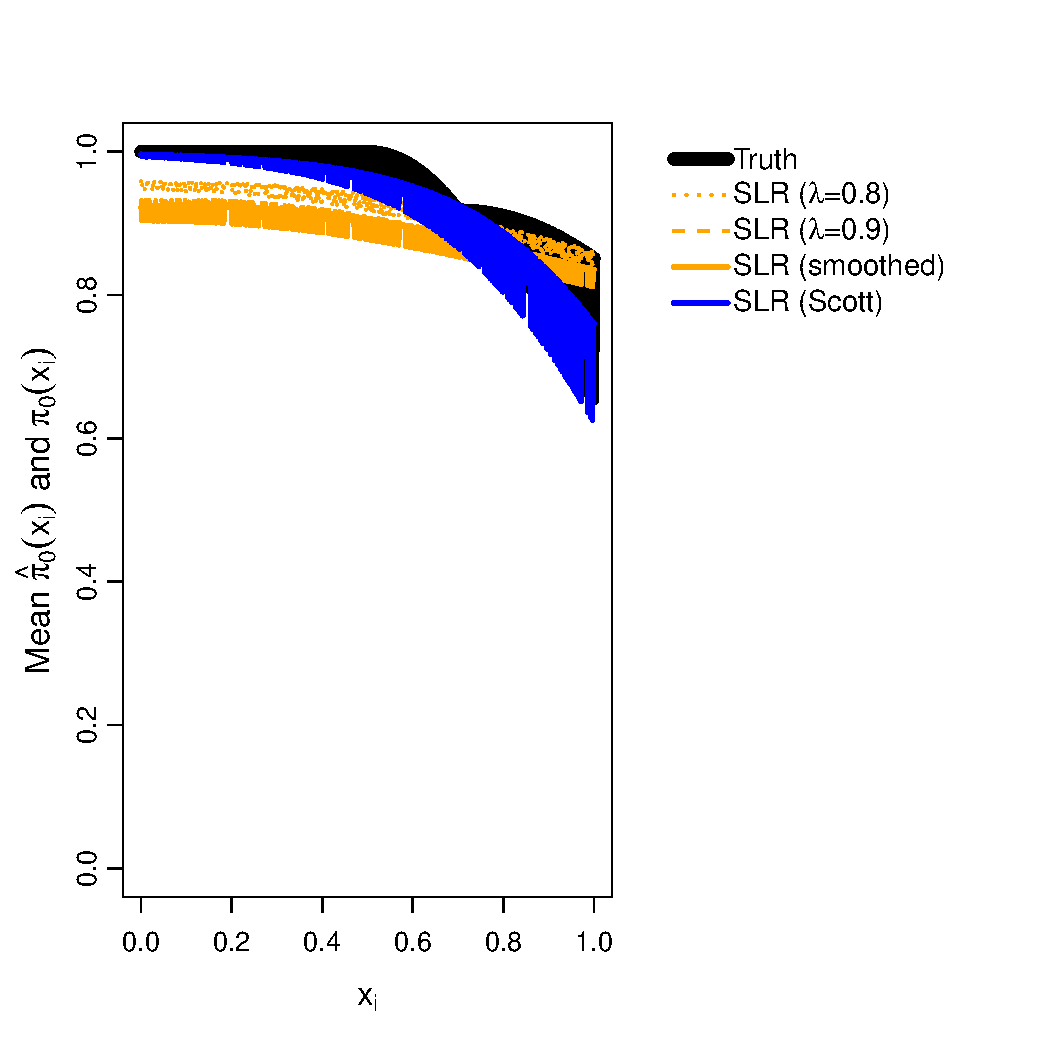
\includegraphics[width=\maxwidth]{Figures/unnamed-chunk-1-4} 
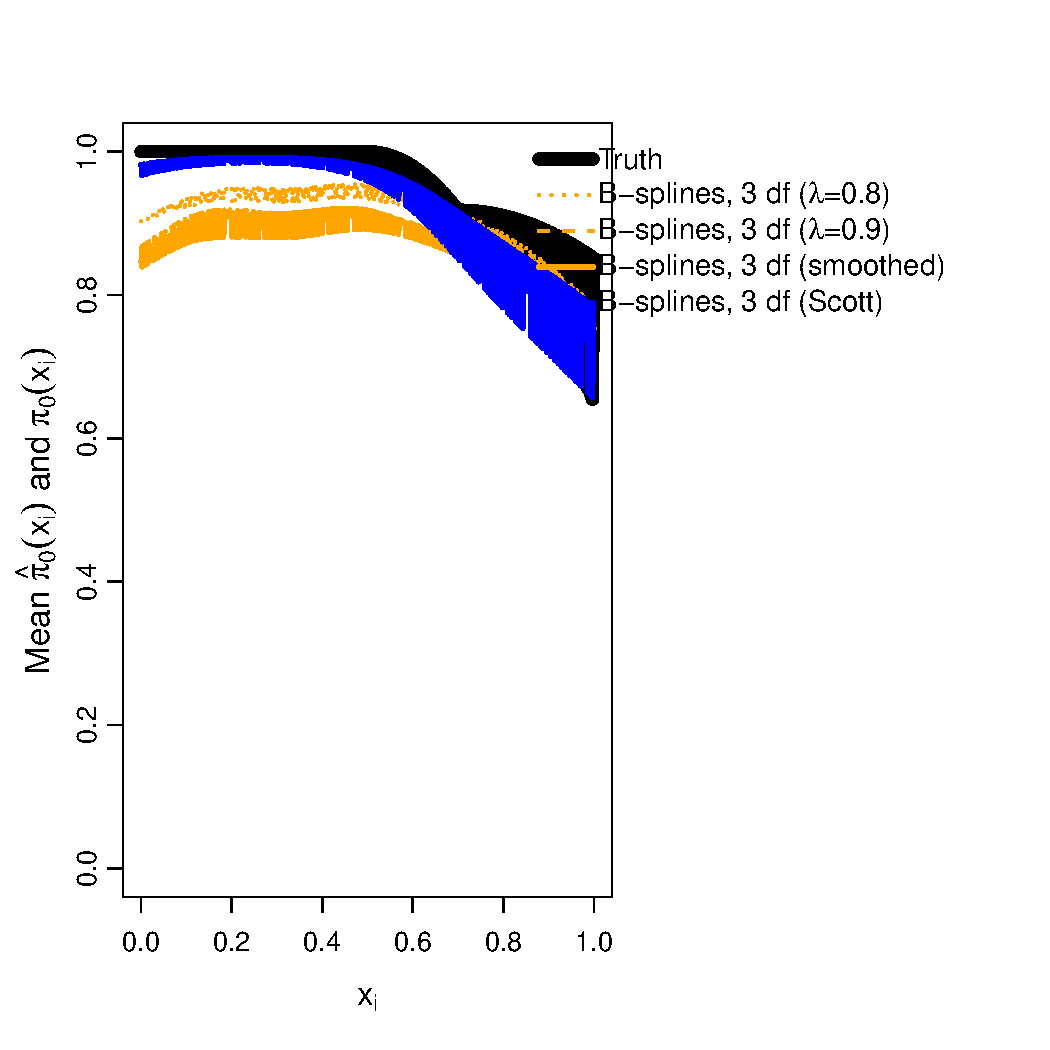
\includegraphics[width=\maxwidth]{Figures/unnamed-chunk-1-5} 
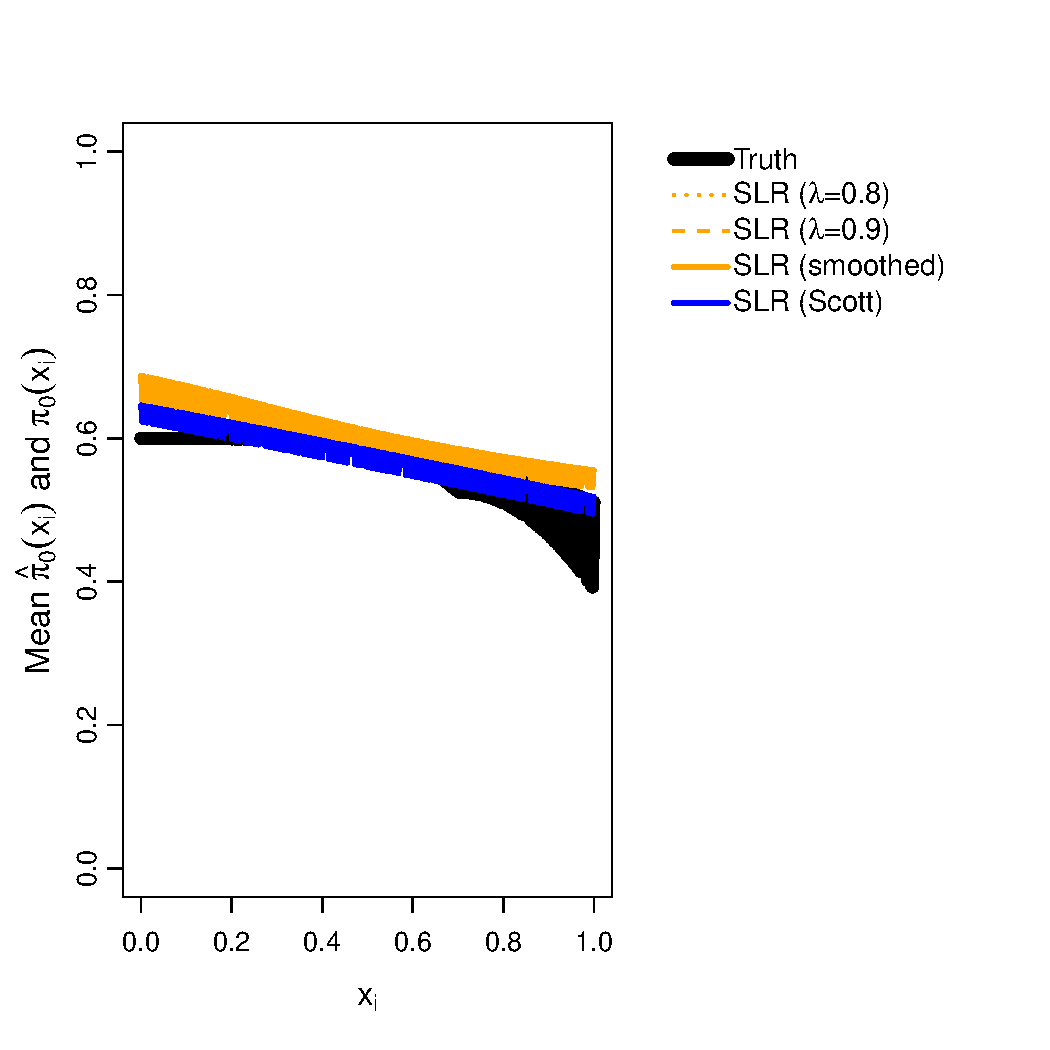
\includegraphics[width=\maxwidth]{Figures/unnamed-chunk-1-6} 
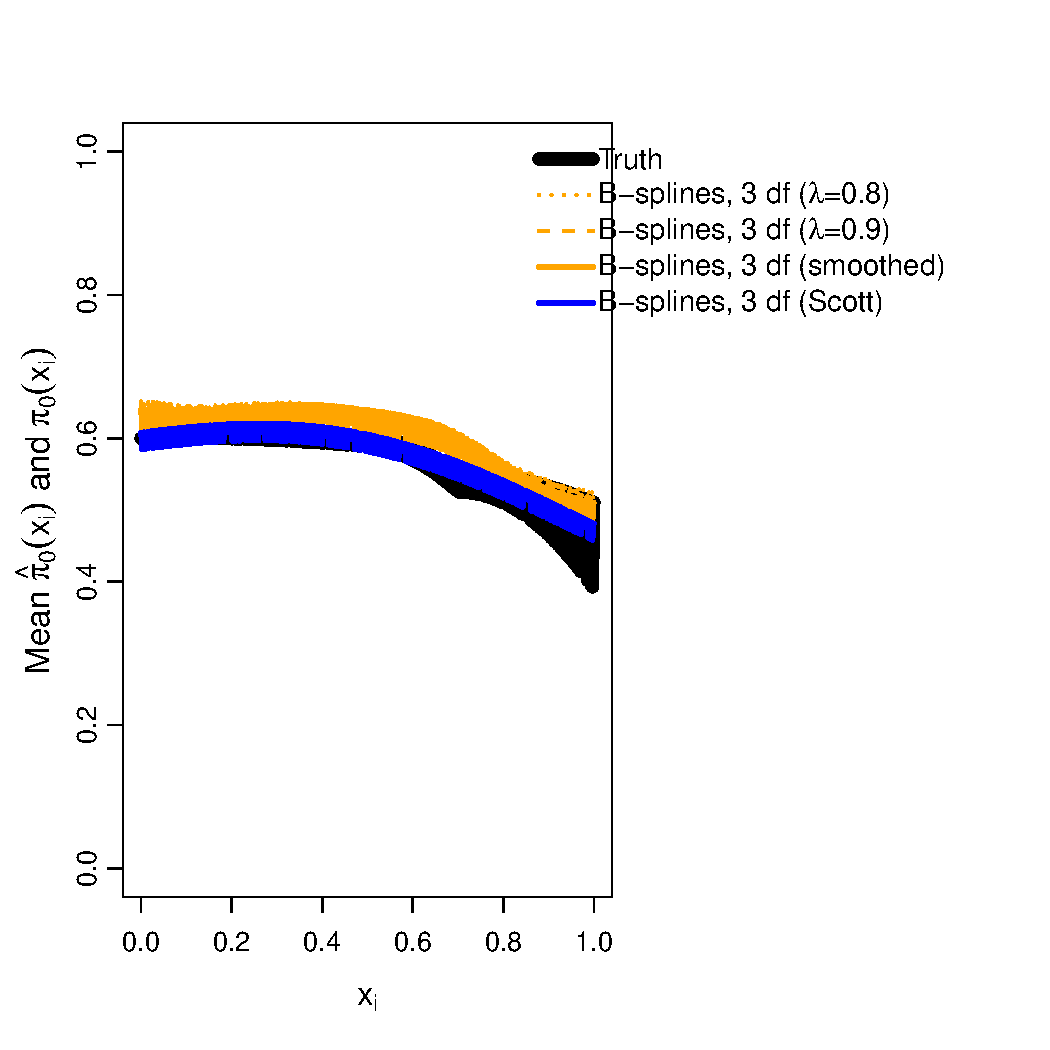
\includegraphics[width=\maxwidth]{Figures/unnamed-chunk-1-7} 
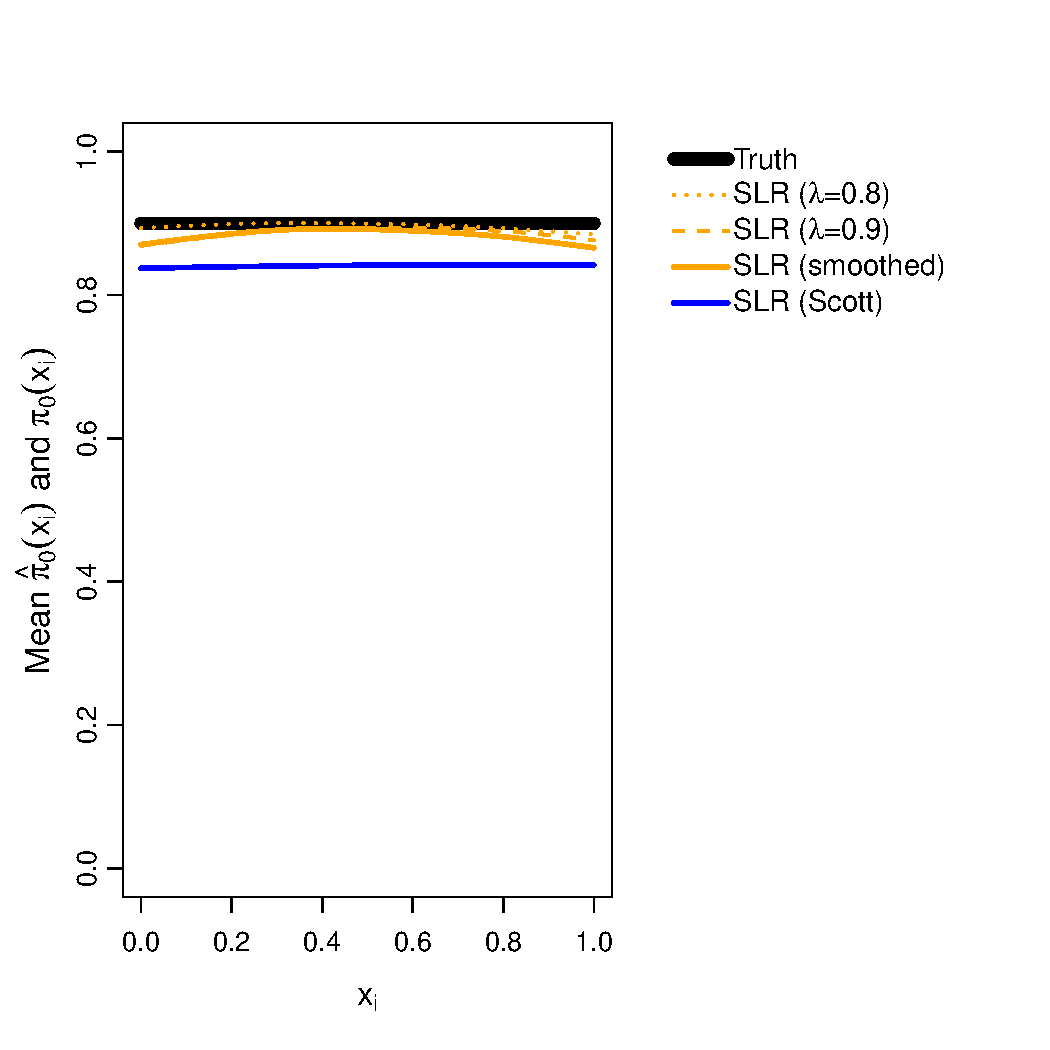
\includegraphics[width=\maxwidth]{Figures/unnamed-chunk-1-8} 
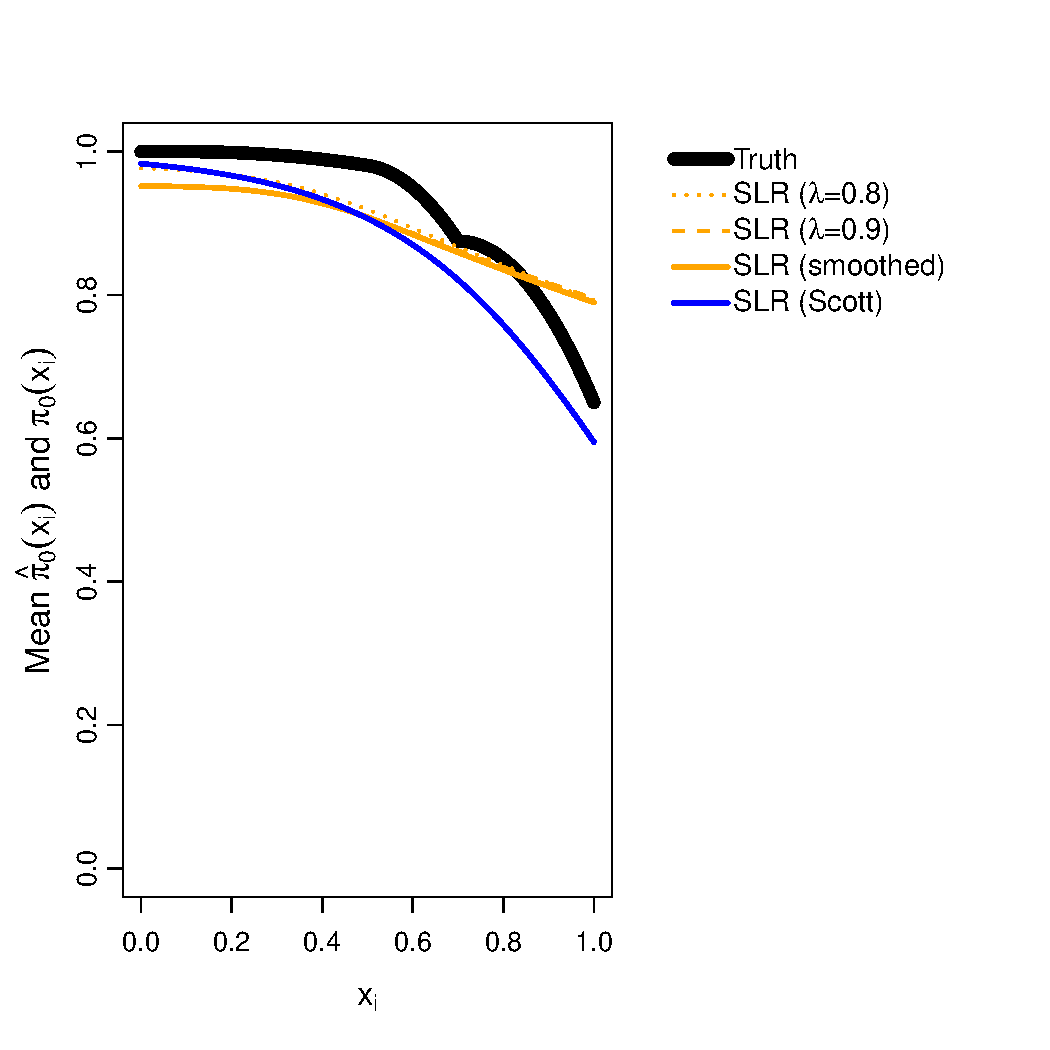
\includegraphics[width=\maxwidth]{Figures/unnamed-chunk-1-9} 
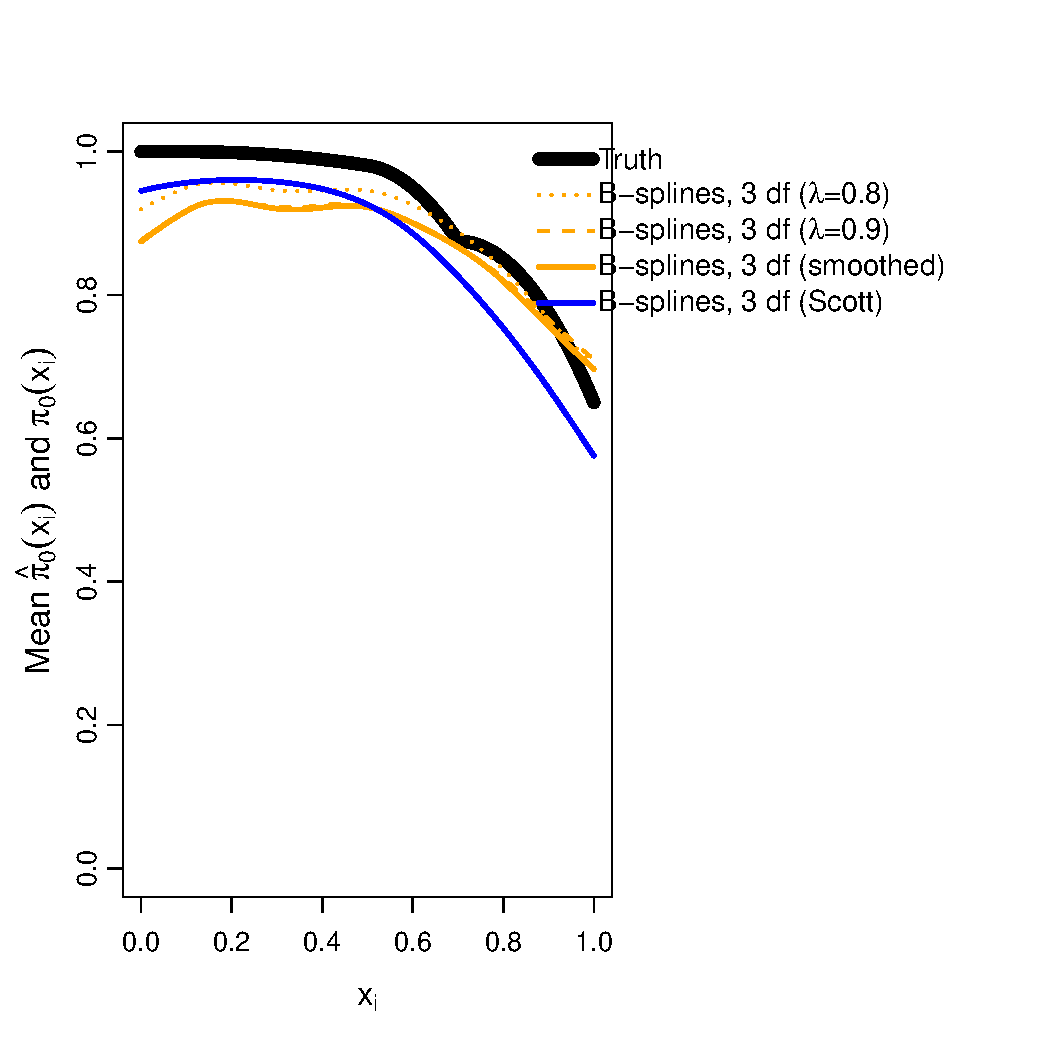
\includegraphics[width=\maxwidth]{Figures/unnamed-chunk-1-10} 
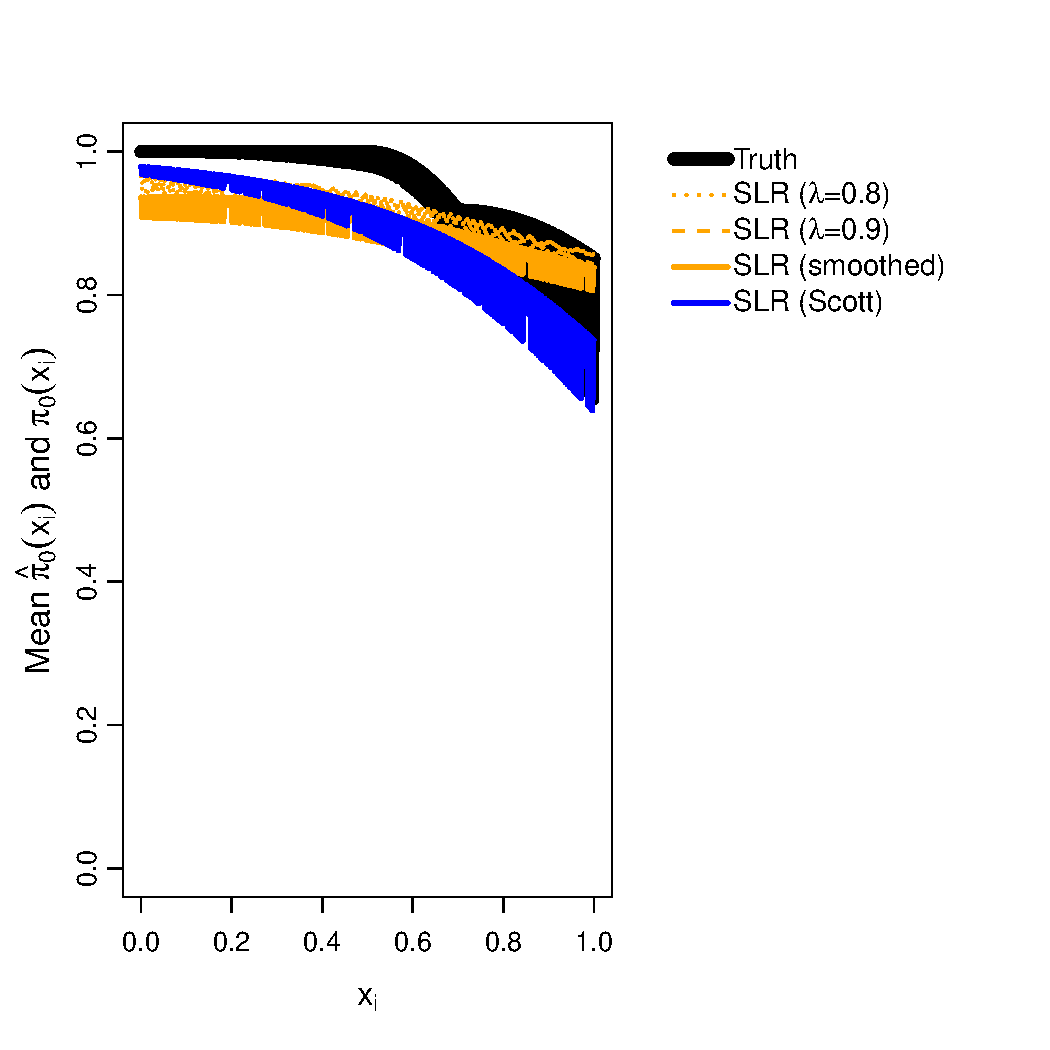
\includegraphics[width=\maxwidth]{Figures/unnamed-chunk-1-11} 
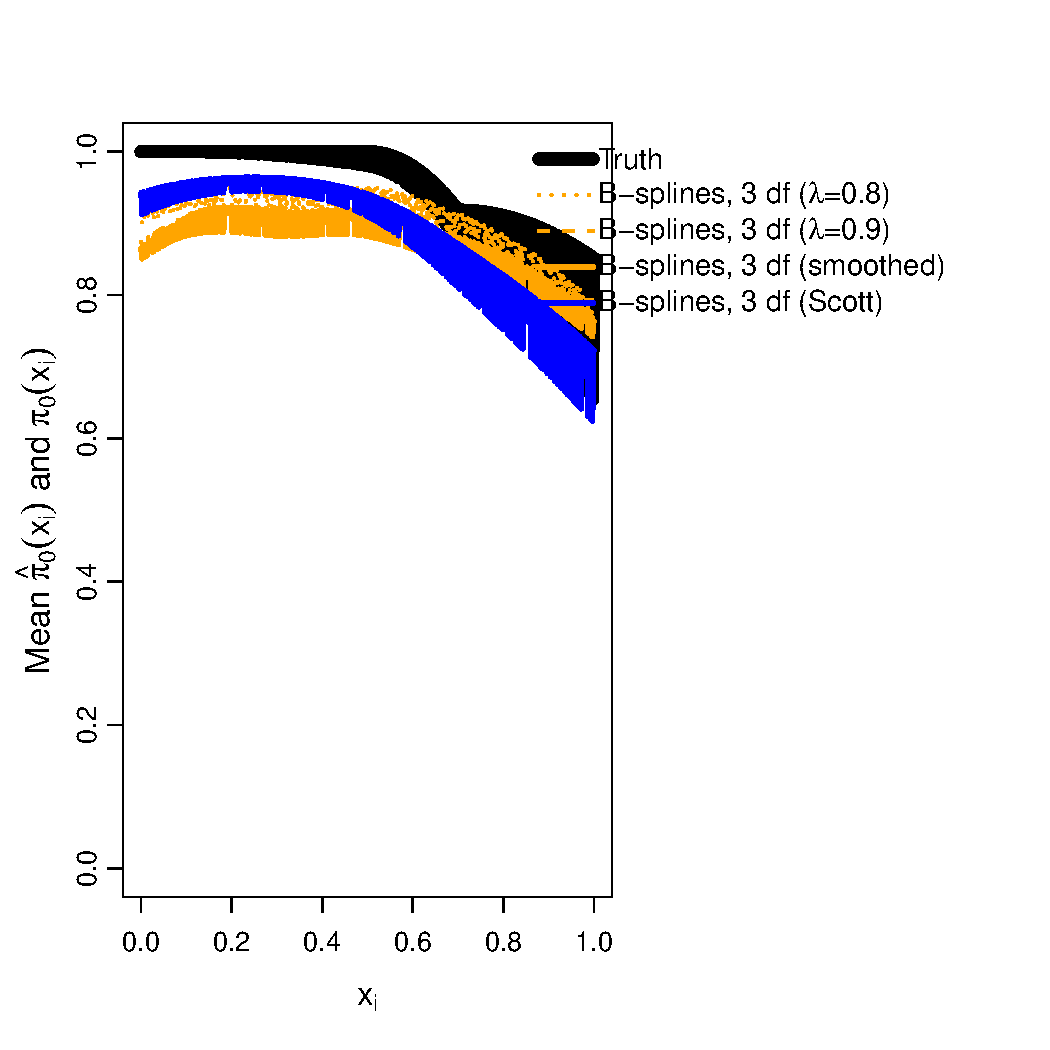
\includegraphics[width=\maxwidth]{Figures/unnamed-chunk-1-12} 
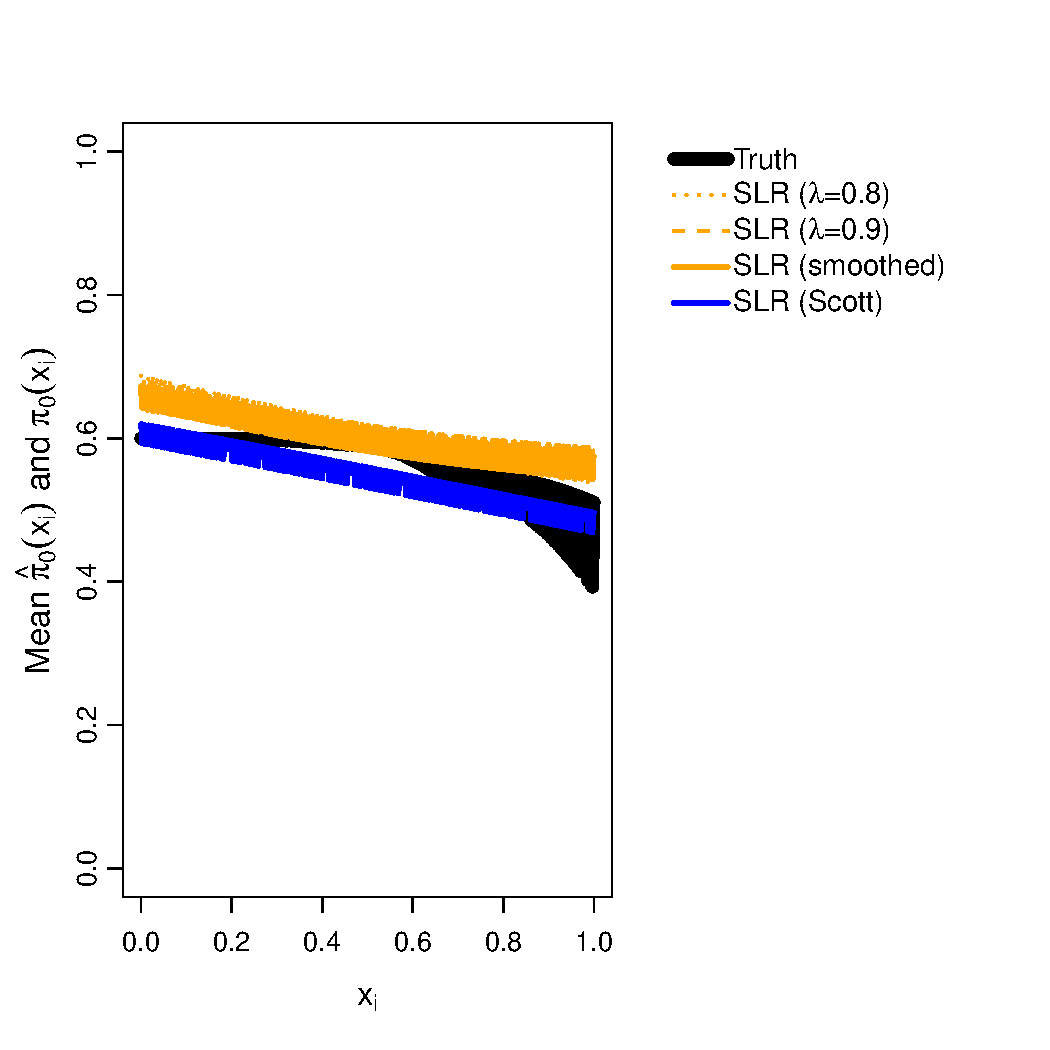
\includegraphics[width=\maxwidth]{Figures/unnamed-chunk-1-13} 
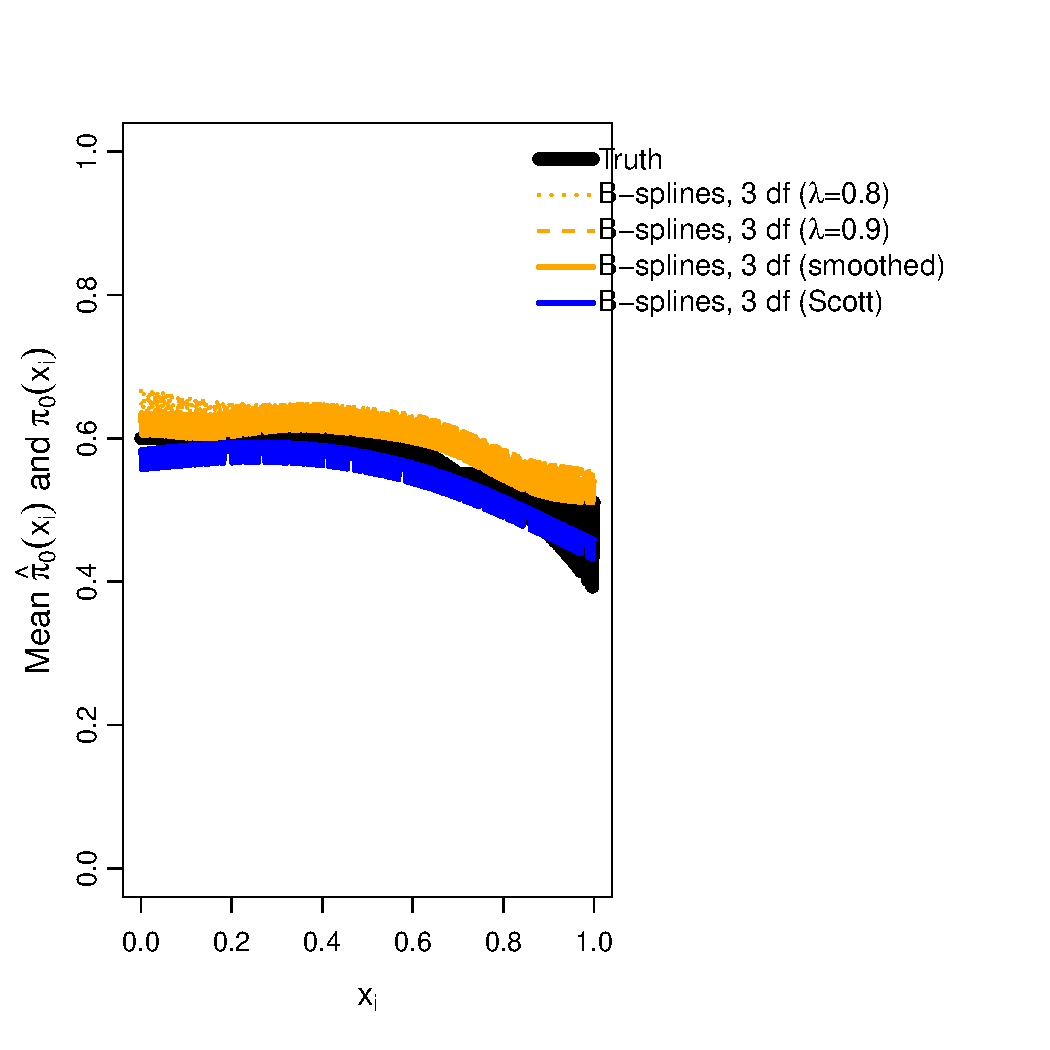
\includegraphics[width=\maxwidth]{Figures/unnamed-chunk-1-14} 

}



\end{knitrout}





Session info:
\begin{knitrout}
\definecolor{shadecolor}{rgb}{0.969, 0.969, 0.969}\color{fgcolor}\begin{kframe}
\begin{alltt}
\hlstd{devtools}\hlopt{::}\hlkwd{session_info}\hlstd{()}
\end{alltt}


{\ttfamily\noindent\itshape\color{messagecolor}{\#\# Session info -----------------------------------------------}}\begin{verbatim}
##  setting  value                       
##  version  R version 3.3.1 (2016-06-21)
##  system   x86_64, mingw32             
##  ui       RTerm                       
##  language (EN)                        
##  collate  English_United States.1252  
##  tz       America/New_York            
##  date     2017-06-16
\end{verbatim}


{\ttfamily\noindent\itshape\color{messagecolor}{\#\# Packages ---------------------------------------------------}}\begin{verbatim}
##  package  * version date       source        
##  devtools   1.12.0  2016-06-24 CRAN (R 3.3.3)
##  digest     0.6.9   2016-01-08 CRAN (R 3.3.1)
##  evaluate   0.10    2016-10-11 CRAN (R 3.3.1)
##  highr      0.6     2016-05-09 CRAN (R 3.3.1)
##  knitr    * 1.15.1  2016-11-22 CRAN (R 3.3.1)
##  magrittr   1.5     2014-11-22 CRAN (R 3.3.1)
##  MASS     * 7.3-45  2016-04-21 CRAN (R 3.3.1)
##  memoise    1.0.0   2016-01-29 CRAN (R 3.3.1)
##  stringi    1.1.1   2016-05-27 CRAN (R 3.3.0)
##  stringr    1.0.0   2015-04-30 CRAN (R 3.3.1)
##  withr      1.0.2   2016-06-20 CRAN (R 3.3.1)
\end{verbatim}
\end{kframe}
\end{knitrout}

\end{document}
